\documentclass[border=16pt]{standalone}
\usepackage{tikz}
\usetikzlibrary{arrows.meta,calc,positioning}
\usepackage{amsmath}

\begin{document}
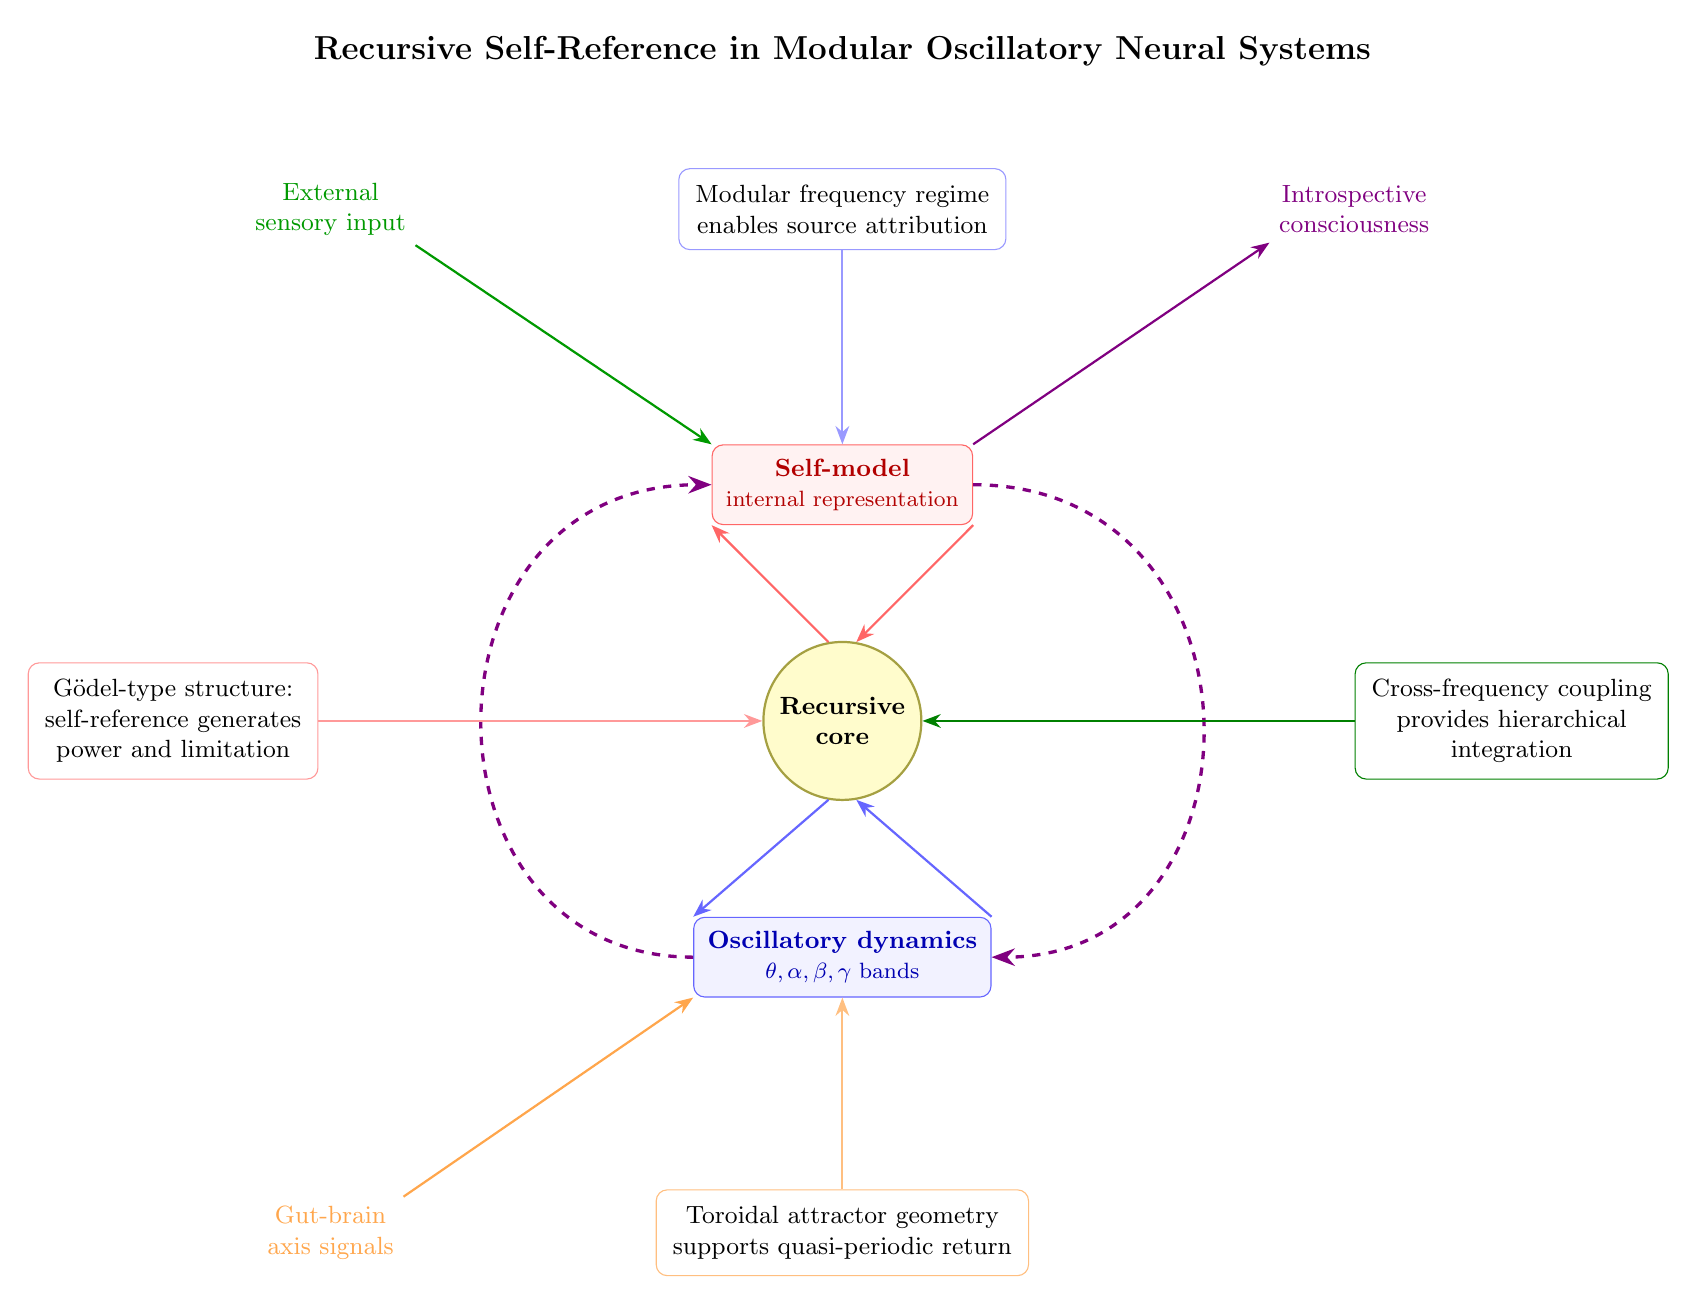
\begin{tikzpicture}[>=Stealth, font=\small,
  outerbox/.style={draw, rounded corners=4pt, inner sep=6pt, align=center, font=\small},
  innerbox/.style={draw, rounded corners=4pt, inner sep=5pt, align=center, font=\small}]

% Title
\node[font=\large\bfseries] at (0,8.5) {Recursive Self-Reference in Modular Oscillatory Neural Systems};

% ============ CENTER: Recursive core ============
\node[circle, fill=yellow!20, draw=yellow!60!black, thick, minimum size=2cm, 
  font=\small\bfseries, align=center] (core) at (0,0) {Recursive\\core};

% ============ INNER RING: Two labeled boxes ============

% Self-model (top)
\node[innerbox, draw=red!60, fill=red!5, minimum width=3cm] (selfmodel) at (0,3.0) 
  {\textbf{\textcolor{red!70!black}{Self-model}}\\
   \textcolor{red!70!black}{\footnotesize internal representation}};

% Oscillatory dynamics (bottom)
\node[innerbox, draw=blue!60, fill=blue!5, minimum width=3.2cm] (oscdyn) at (0,-3.0) 
  {\textbf{\textcolor{blue!70!black}{Oscillatory dynamics}}\\
   \textcolor{blue!70!black}{\footnotesize $\theta, \alpha, \beta, \gamma$ bands}};

% Arrows between core and inner ring boxes
\draw[->, thick, red!60] (core.100) -- (selfmodel.south west);
\draw[->, thick, red!60] (selfmodel.south east) -- (core.80);

\draw[->, thick, blue!60] (core.260) -- (oscdyn.north west);
\draw[->, thick, blue!60] (oscdyn.north east) -- (core.280);

% Dashed recursive loop arrows (wide, going far outside to avoid all boxes)
\draw[->, very thick, violet, dashed] 
  (selfmodel.east) .. controls (5.5,3.0) and (5.5,-3.0) .. (oscdyn.east);

\draw[->, very thick, violet, dashed] 
  (oscdyn.west) .. controls (-5.5,-3.0) and (-5.5,3.0) .. (selfmodel.west);

% ============ OUTER RING: Four concept boxes ============

% Top: Modular frequency regime
\node[outerbox, draw=blue!40, fill=white] (modfreq) at (0,6.5) 
  {Modular frequency regime\\enables source attribution};
\draw[->, thick, blue!40] (modfreq.south) -- (selfmodel.north);

% Bottom: Toroidal attractor
\node[outerbox, draw=orange!50, fill=white] (torus) at (0,-6.5) 
  {Toroidal attractor geometry\\supports quasi-periodic return};
\draw[->, thick, orange!50] (torus.north) -- (oscdyn.south);

% Right: Cross-frequency coupling (pushed further right)
\node[outerbox, draw=green!50!black, fill=white] (crossfreq) at (8.5,0) 
  {Cross-frequency coupling\\provides hierarchical\\integration};
\draw[->, thick, green!50!black] (crossfreq.west) -- (core.east);

% Left: Godel analogy (pushed further left)
\node[outerbox, draw=red!40, fill=white] (godel) at (-8.5,0) 
  {G\"odel-type structure:\\self-reference generates\\power and limitation};
\draw[->, thick, red!40] (godel.east) -- (core.west);

% ============ EXTERNAL INPUTS ============

% External sensory input (top-left, angled to avoid overlap)
\node[font=\small, green!60!black, align=center] (sensinput) at (-6.5,6.5) {External\\sensory input};
\draw[->, thick, green!60!black] (sensinput.south east) -- (selfmodel.north west);

% Gut-brain axis (bottom-left, angled)
\node[font=\small, orange!70, align=center] (gutbrain) at (-6.5,-6.5) {Gut-brain\\axis signals};
\draw[->, thick, orange!70] (gutbrain.north east) -- (oscdyn.south west);

% Output: Introspective consciousness (top-right)
\node[font=\small, violet, align=center] (introsp) at (6.5,6.5) {Introspective\\consciousness};
\draw[->, thick, violet] (selfmodel.north east) -- (introsp.south west);

\end{tikzpicture}
\end{document}
